\documentclass[10pt,twocolumn,letterpaper]{article}

\usepackage{cvpr}
\usepackage{times}
\usepackage{epsfig}
\usepackage{graphicx}
\usepackage{amsmath}
\usepackage{amssymb}
\usepackage{url}

% Include other packages here, before hyperref.

% If you comment hyperref and then uncomment it, you should delete
% egpaper.aux before re-running latex.  (Or just hit 'q' on the first latex
% run, let it finish, and you should be clear).
%\usepackage[pagebackref=true,breaklinks=true,letterpaper=true,colorlinks,bookmarks=false]{hyperref}

\cvprfinalcopy % *** Uncomment this line for the final submission

\def\cvprPaperID{****} % *** Enter the 3DV Paper ID here
\def\httilde{\mbox{\tt\raisebox{-.5ex}{\symbol{126}}}}

% Pages are numbered in submission mode, and unnumbered in camera-ready
\setcounter{page}{4321}
\begin{document}

%%%%%%%%% TITLE
\title{3D Object Recognition with Deep Networks}

\author{Adrian Schneuwly\\
{\tt\small adrischn@ethz.ch}
\and
Johannes Oswald\\
{\tt\small voswaldj@eth.ch}
\and
Tobias Grundmann\\
{\tt\small tobiagru@ethz.ch}
}

\maketitle
% \thispagestyle{empty}

%%%%%%%%% ABSTRACT
\begin{abstract}
   The increasing amount of LiDAR and RGBD cameras in e.g. mobile devices
   and robotic systems provide us with new information which can aid in various task including object recognition. In this paper we will discribe 3D Convolutional Deep Neural Networks and  how they are trained to recognize voxelized point cloud data from common objects.
\end{abstract}
%%%%%%%%% BODY TEXT

\section{Introduction}

One of the crucial tasks of computer systems based on visual information e.g. self-driving cars, autonomous robots, virtual enviroments ( Figure \ref{fig:obj_rec}) is to get a semantic understanding of the enviroment. Depth data has already proved its usability in obstacle avoidance or mapping but we want to investigate its potential to improve object recognition.

%% include figure of udacity

Since Deep Learning dramatically improved state of the art object recognition \cite{cnn}, we will use Neural Networks to recognize objects from given point clouds. Especially the idea behind convolution in 2D Object recognition will be translated to our 3D data, resulting in a fast and accurate detector. 

\begin{figure}[h]
	\label{fig:obj_rec}
	\centering
	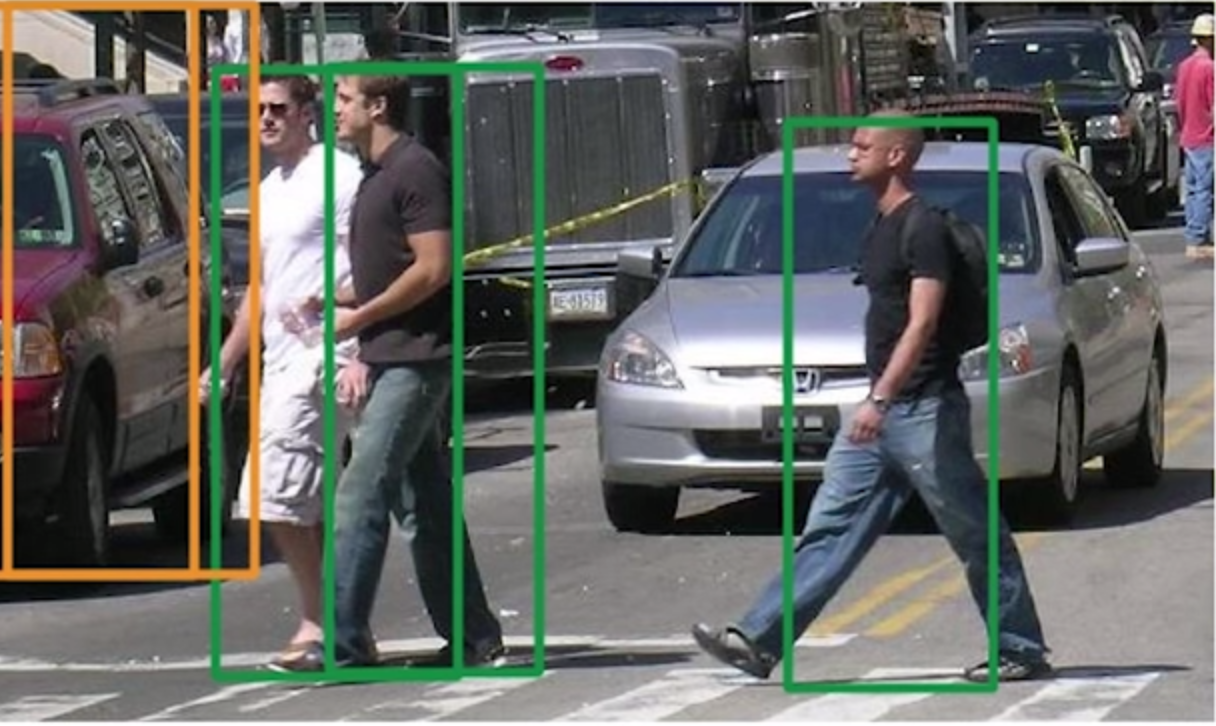
\includegraphics[width=0.45\textwidth]{obj_rec}
	\caption{Example of object recognitions. Source: \cite{udacity}}
\end{figure}

%-------------------------------------------------------------------------

\section{Related Work}

On the one hand, There is a large body of work of object recognition using 3D point clouds but not making use of Neural Networks. 
Mostly methods combine hand-crafted features or descriptors with a machine learning classifier ([10], [11], [12]). 
Similiar methods are seen with semantic segmentation, with structured output classifiers instead of single output classifiers ([14], [15], [16]).

On the other hand 2.5D CNNs were used for object recognition but fail to make full use of geometric information in the data. Their approaches simply treat the depth channel as an additional channel, along with the RGB channels. ([17], [18], [19], [20]) 

Additionally, 3D CNNs already proved there usability in video analysis ([23], [24]). In this case, time acts as the third dimension but algorithmically, these architectures work the same as ours, but the nature of the data is very different.

\textbf{Das so machen? ist quasi kopiert von VoxNet. Finde ich ok, mir egal}

\section{Convolutional Neural Networks}

At the core of a neural network is a logistic classifier. 
For given data, we train weights and bias of a linear equation which will then be transformed into 
probabilites by using a softmax function. 

\begin{figure}[h]
	\label{fig:classifier}
	\centering
	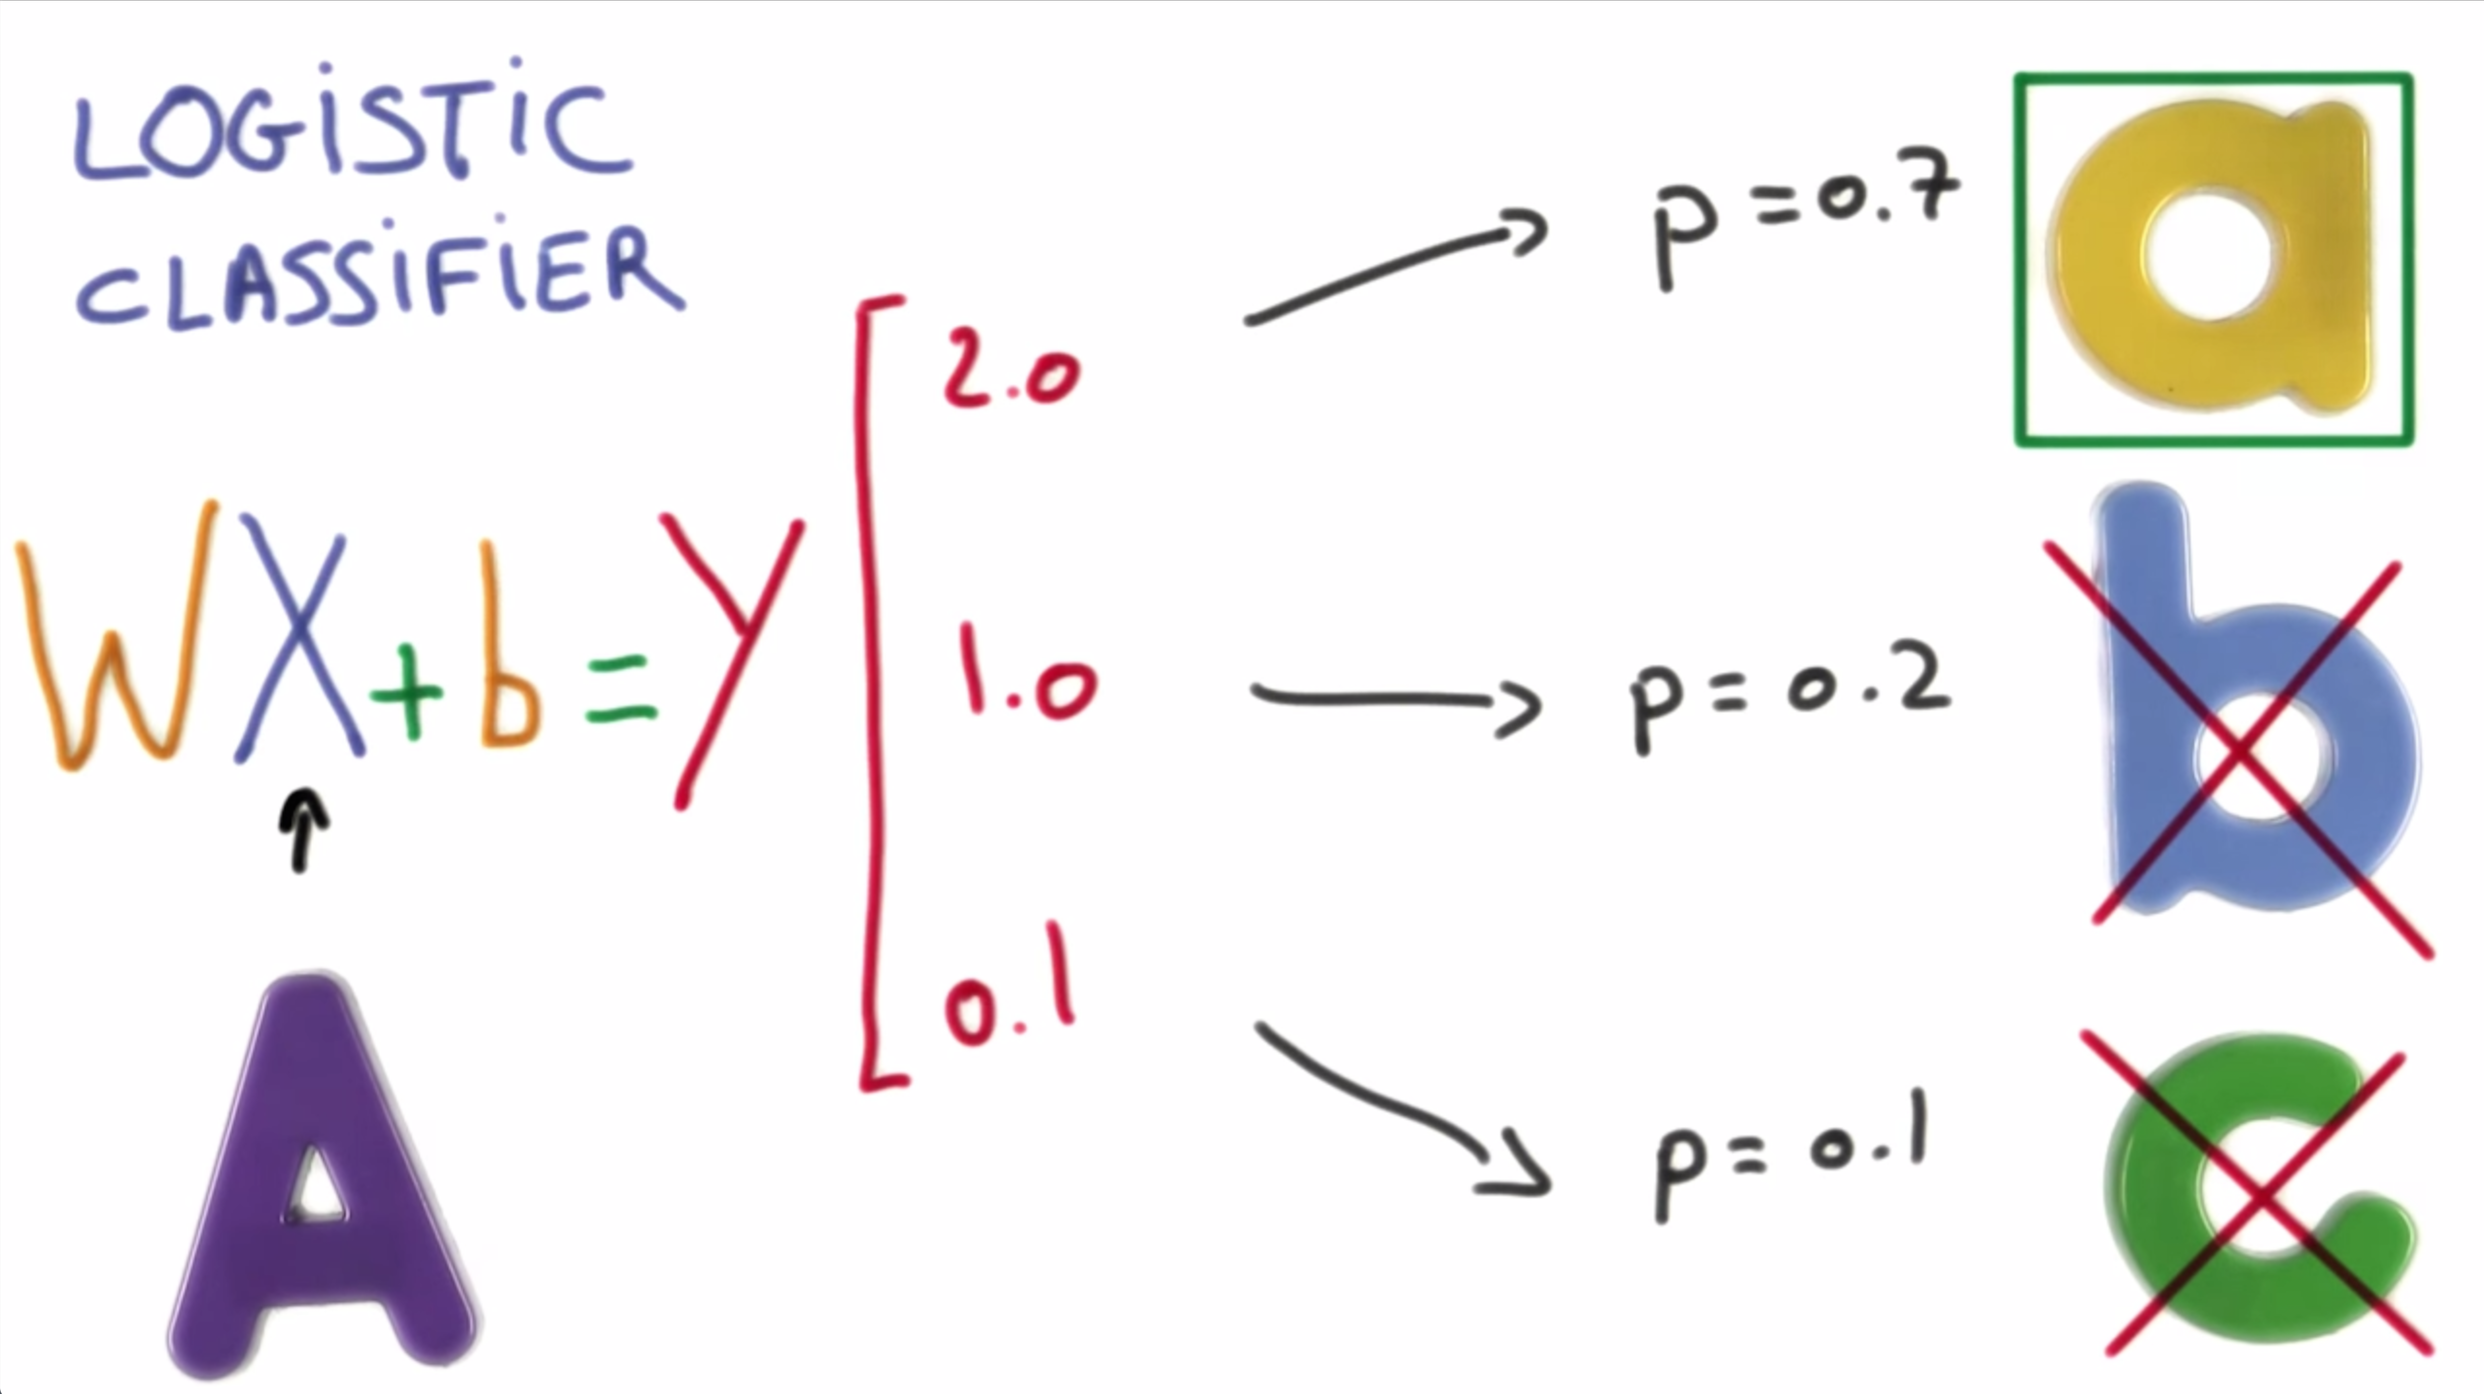
\includegraphics[width=0.4\textwidth]{classifier}
	\caption{Weight and bias (W,b) get trained to classify input A. Source: \cite{udacity}}
\end{figure}

Linear models are limited and therefore we deepen the network in our case through convolutions and max pooling.
For convolution we define a patch which then walks through our 3D Data and runs a small neural network on this patch with given output size / depth. When leaving out /jumping voxels (striding), the spatial dimension is squeezed while extracting local features of the given object. 
Through repeating this procedure we arrive at an output depth which coresponds to a similiar semantic complexity of our representation. 

\begin{figure}[h]
	\label{fig:convolution}
	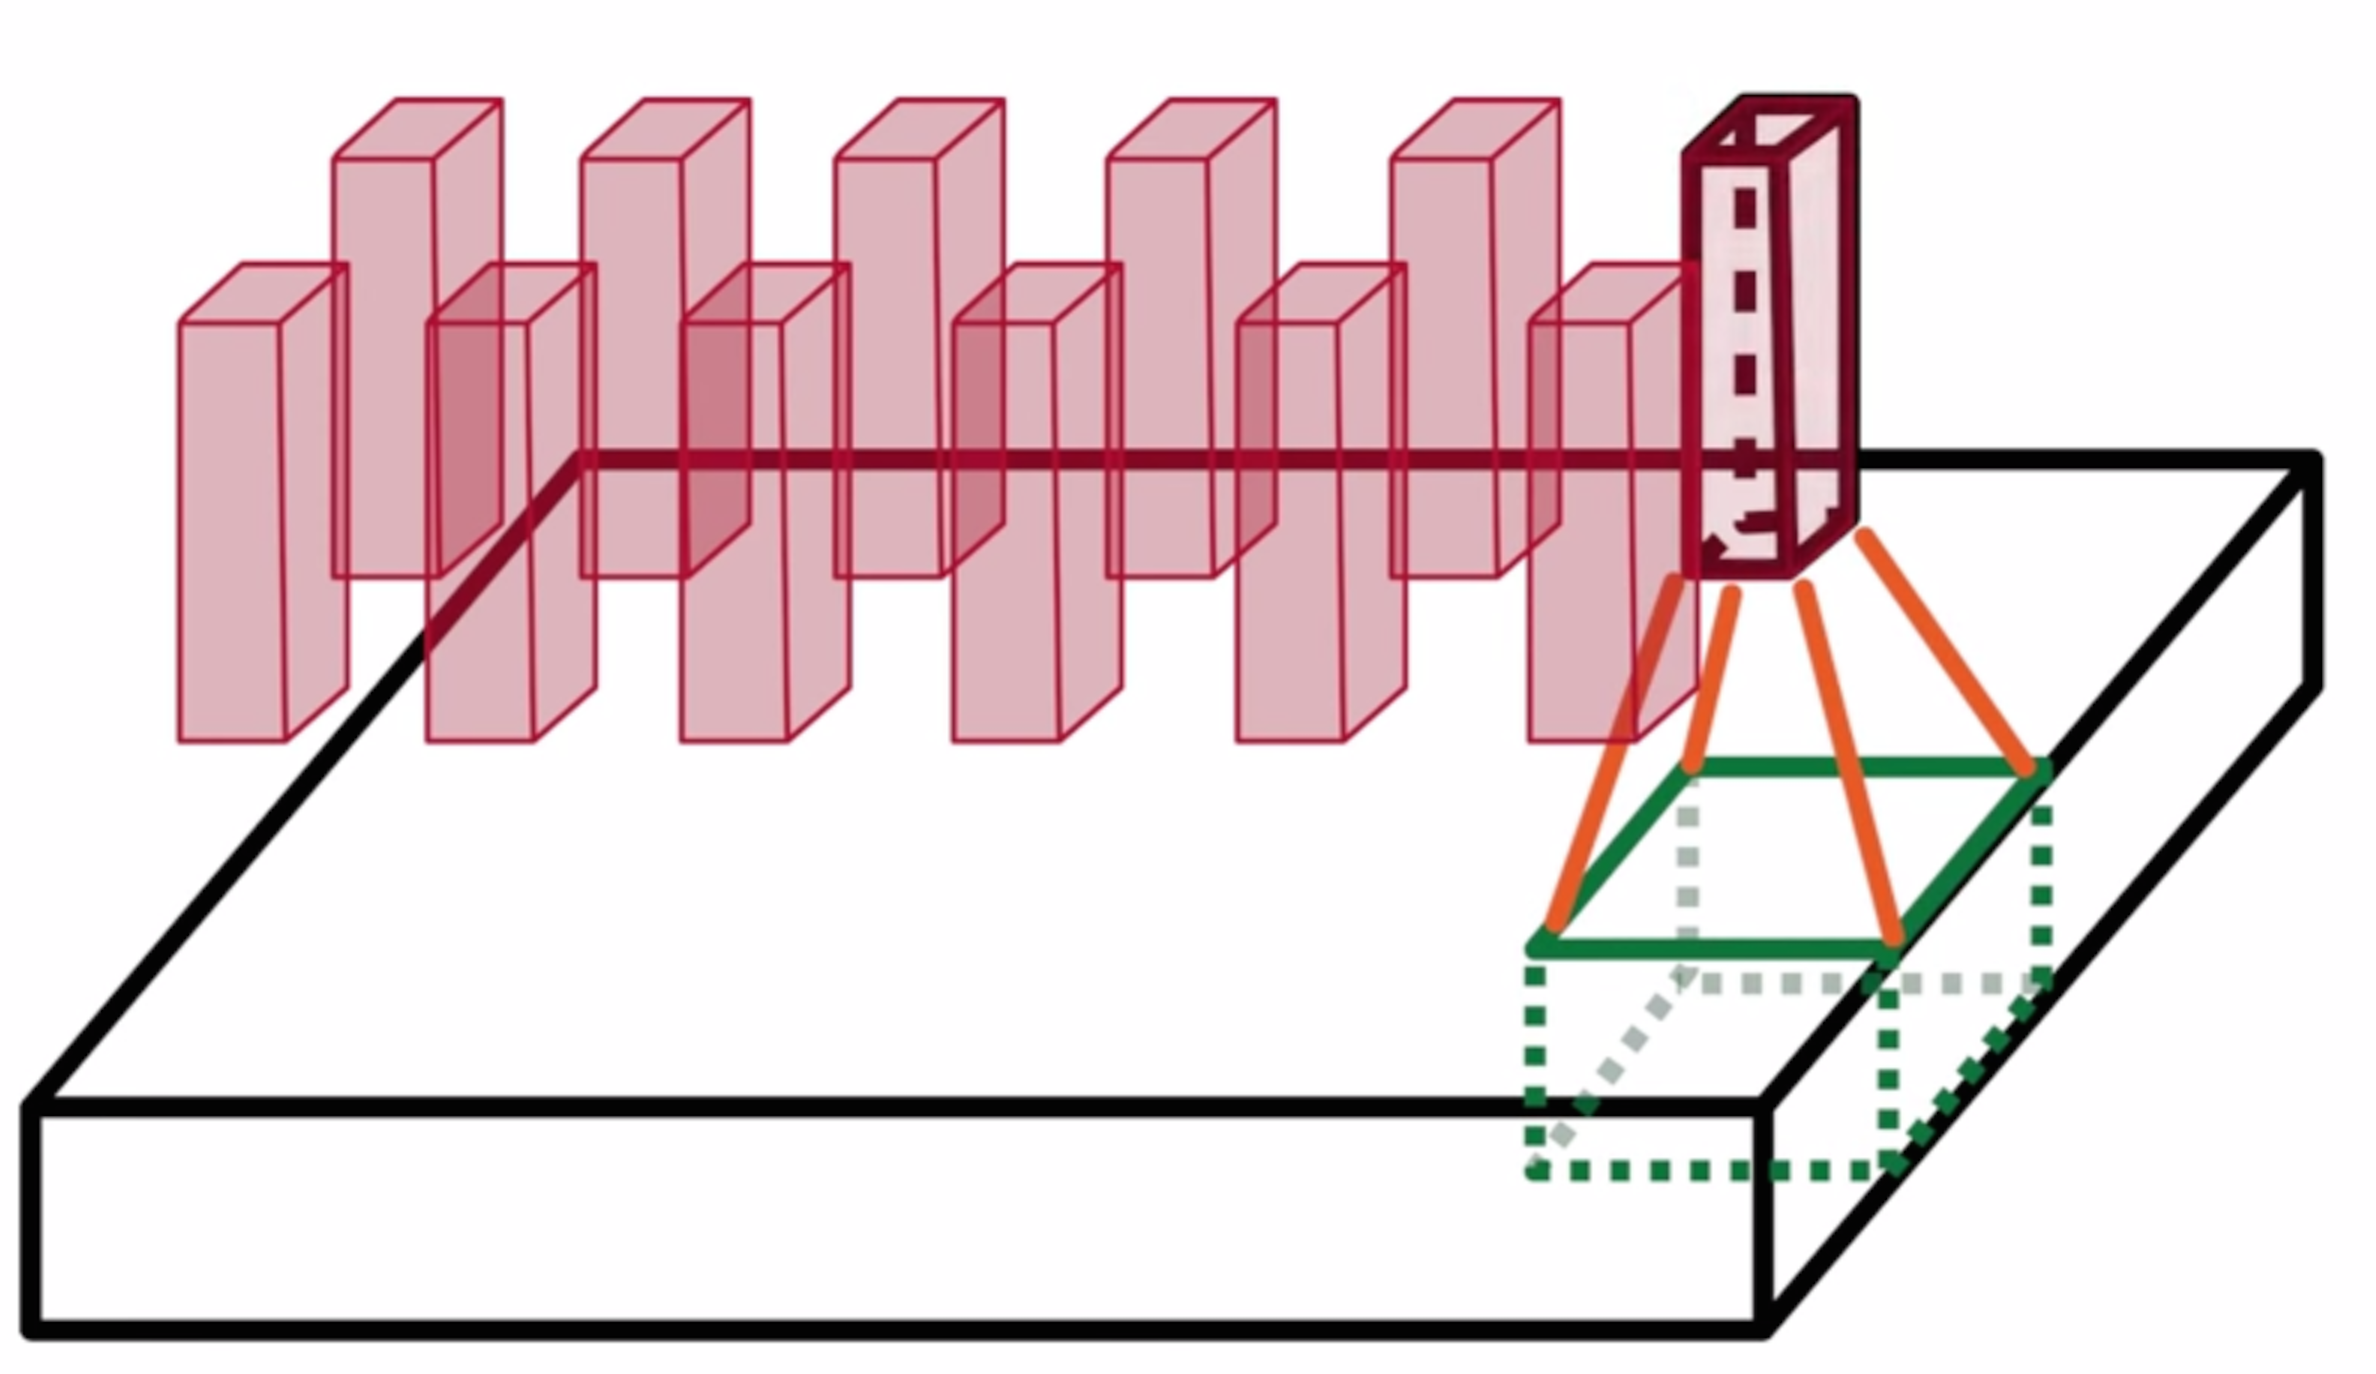
\includegraphics[width=0.2\textwidth]{conv}
	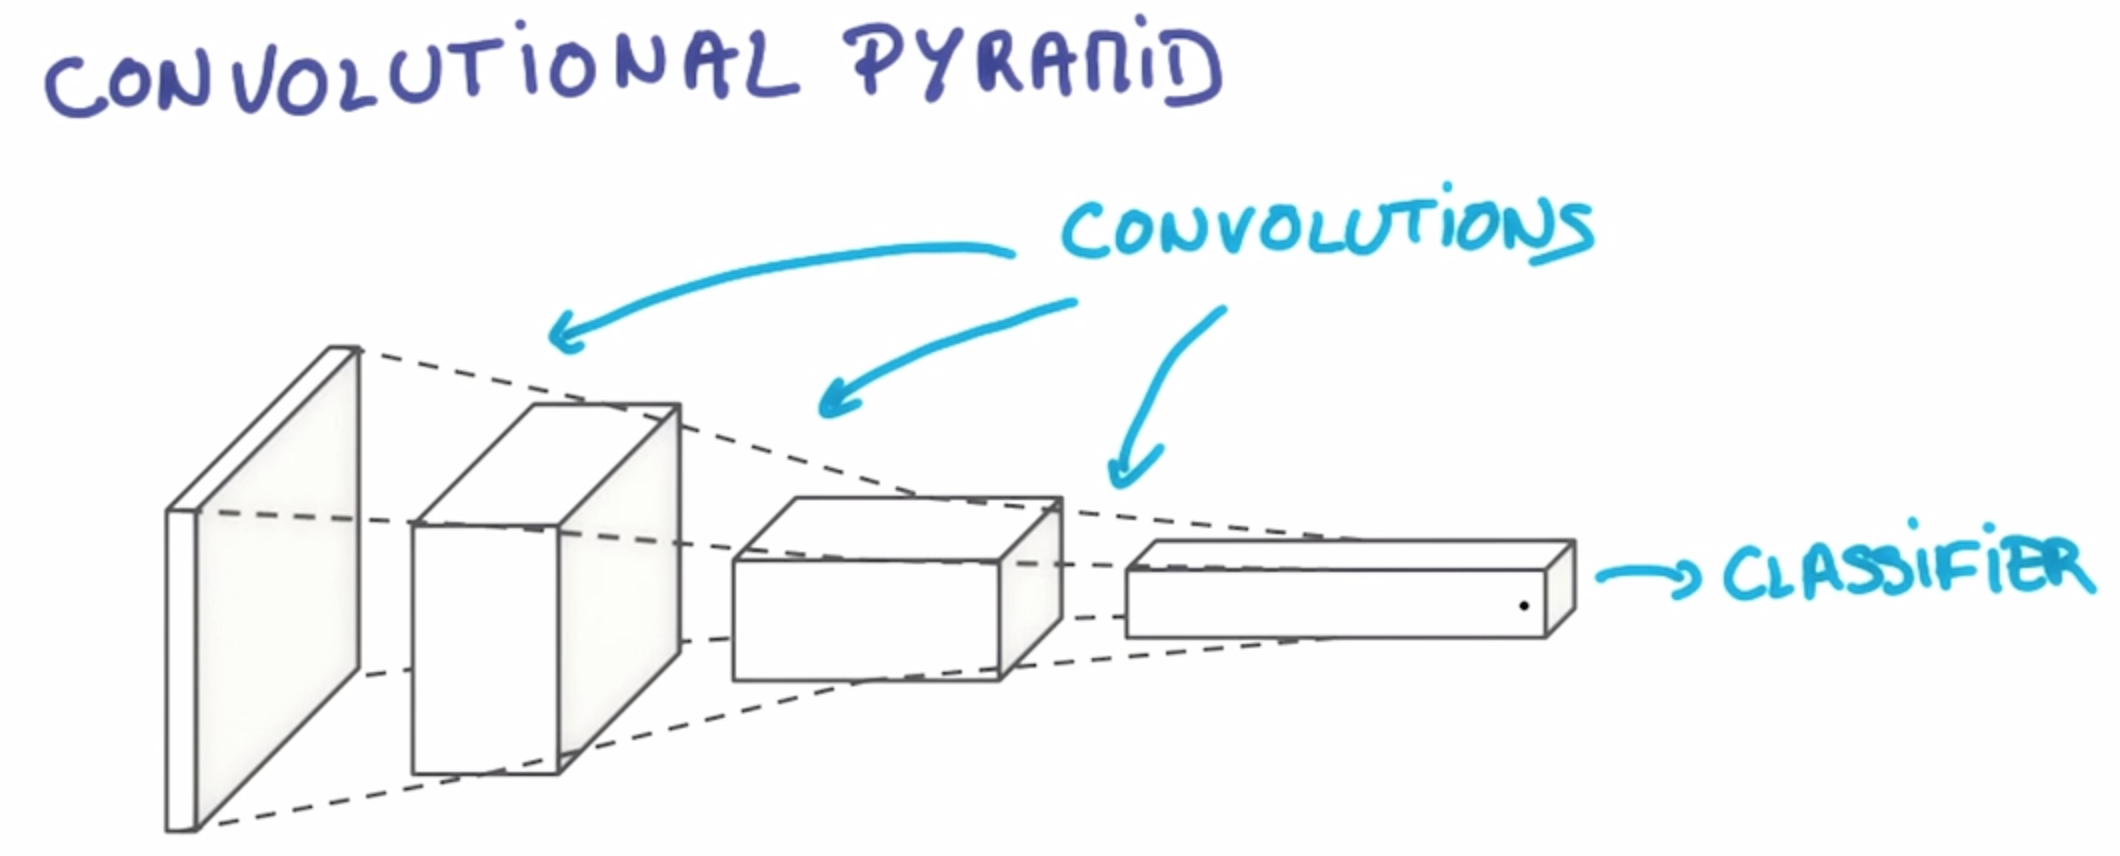
\includegraphics[width=0.3\textwidth]{pyra}
	\caption{Left: Patch with stride 2 \quad Right: Multiple Covolutions. Source: \cite{udacity}}
\end{figure}

The second technique to deepen our network is pooling. Instead of striding to sqeeze our dimension, we can extract e.g. the maximum of a patch and therefore reduce spatial dimension. See detailed discribition of model used in our approach in Figure \ref{fig:model}.

\begin{figure}[h]
	\label{fig:pooling}
	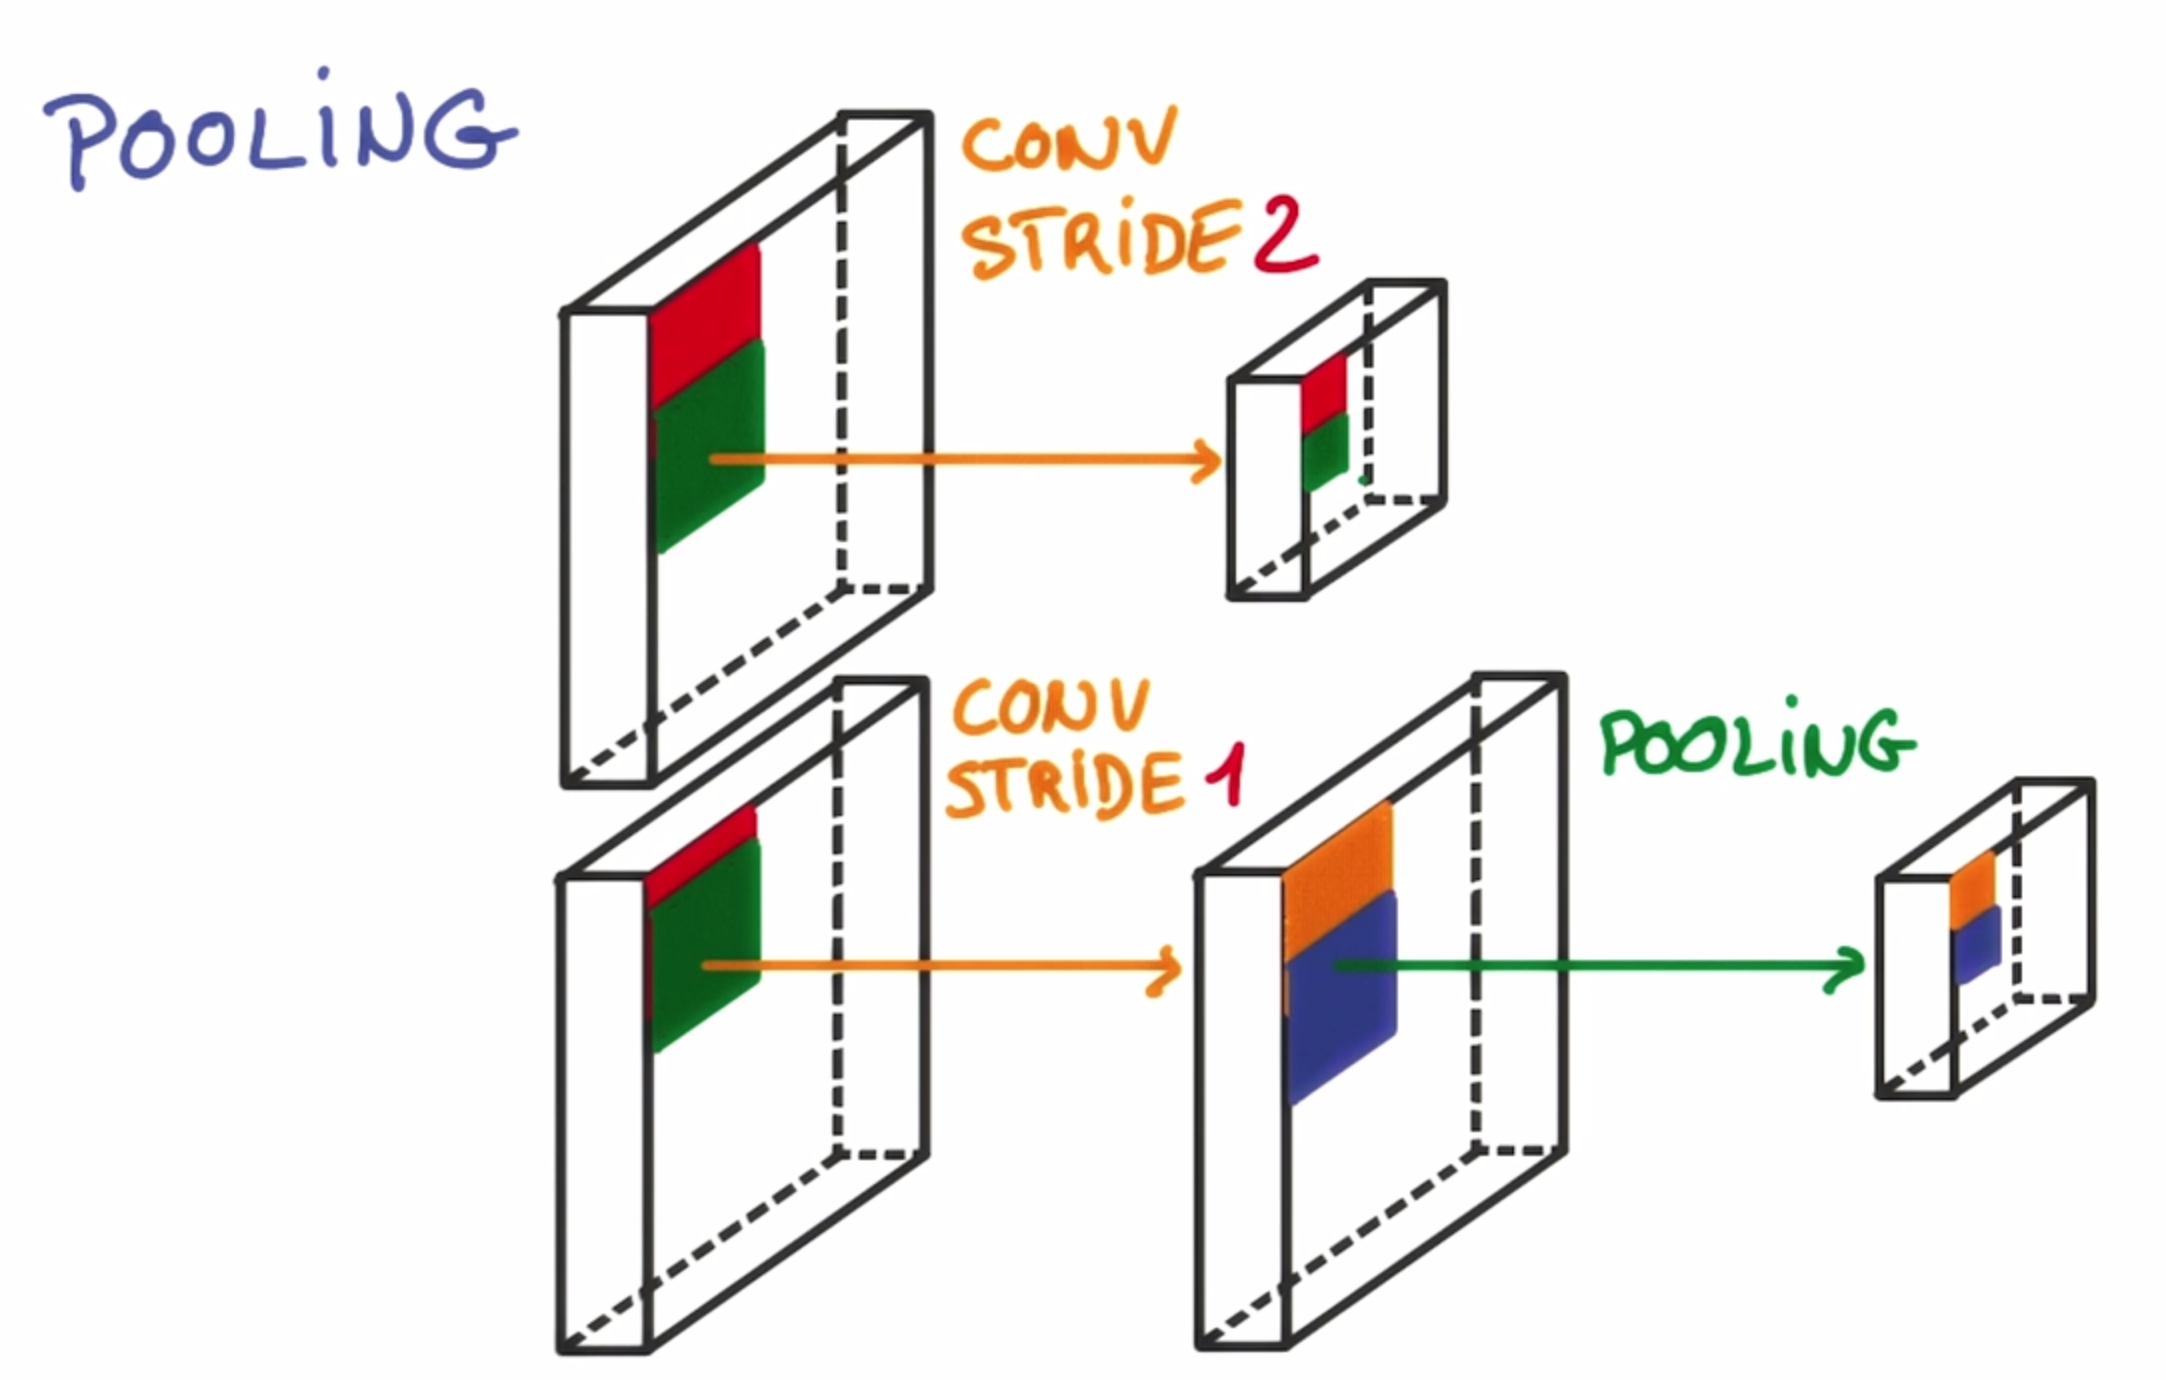
\includegraphics[width=0.25\textwidth]{con_max}
	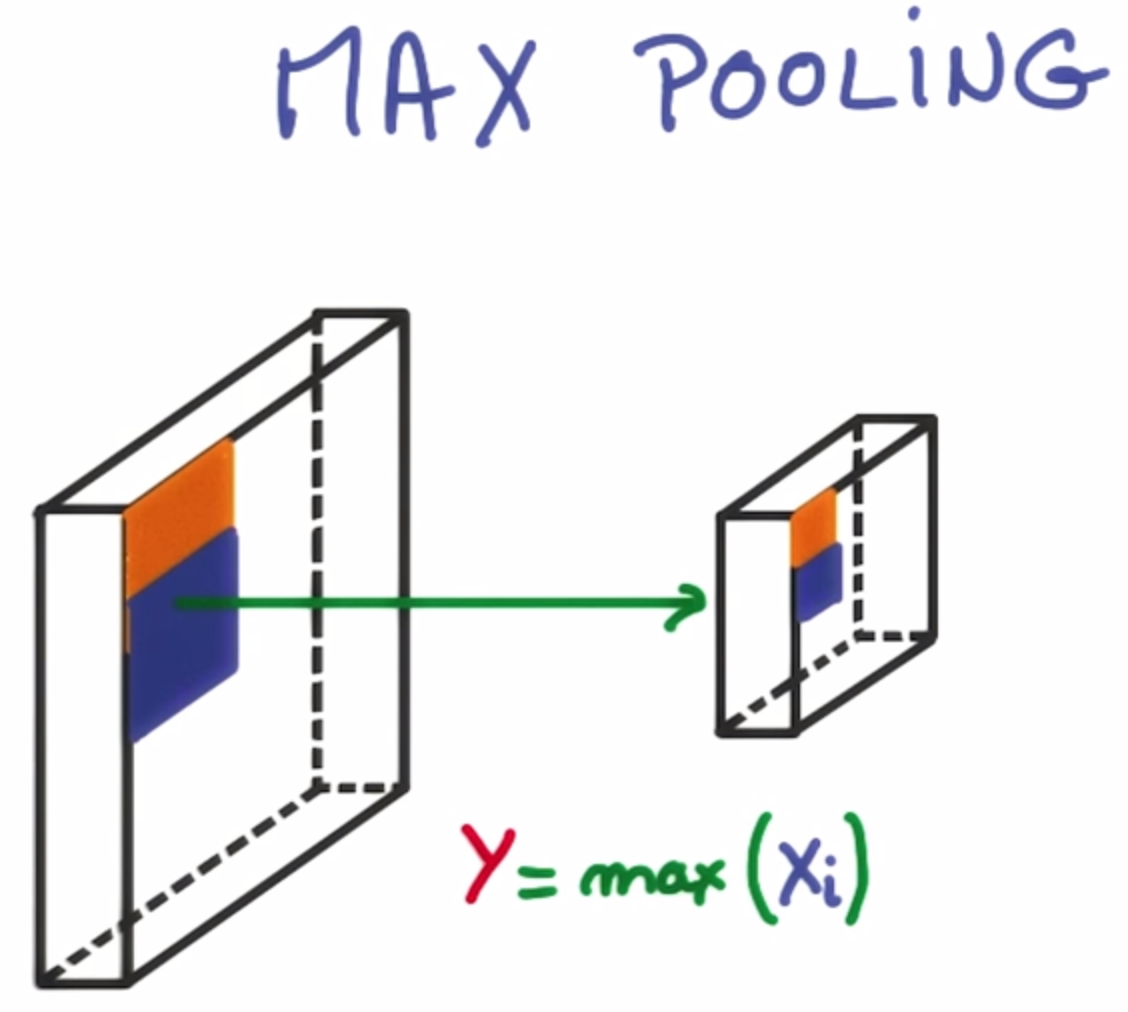
\includegraphics[width=0.16\textwidth]{max}
	\caption{Left: Stride 2 vs. Stride 1 + Pooling \quad Right: Max-Pooling. Source: \cite{udacity}}
\end{figure}

In order to train our model, we have to test how well it is doing during and after training. 
Testing the model on the data we trained it with does not work since the model remembers input data so we split the data into test- and training set which gives us accurate results how well the classifier is doing on unknown data. This common phenomenon, that a complex model fits a given dataset but fails to generalizes on new data, is called \textit{overfitting}.

\section{Data: Princeton ModelNet}

The data on which we train our Deep Network was build by \cite{shape}. After a list of the most
common object categories in the world was compiled from Princtons SUN database \cite{sun}, 3D CAD models were collected through online 
search engines. To verify the object assigment to each category, human workers on Amazon Mechanical Turk were hired to validate manually. We trained our neural network on one smaller and one larger dataset containing 10 respectivally 40 categories which each ?XXXX? objects.

\section{Reimplementing: VoxNet \cite{maturana_iros_2015}}

\textit{In the following, parts contributed by Author 1/2/3 will be labeled 
as A1/A2/A3.}

Overall Goal is to classify an object from a given point cloud. After voxilizing to format 32x32x32, we train our CNN on these occupancy grids, Figure \ref{fig:algo}.

\begin{figure}[h]
	\label{fig:algo}
	\centering
	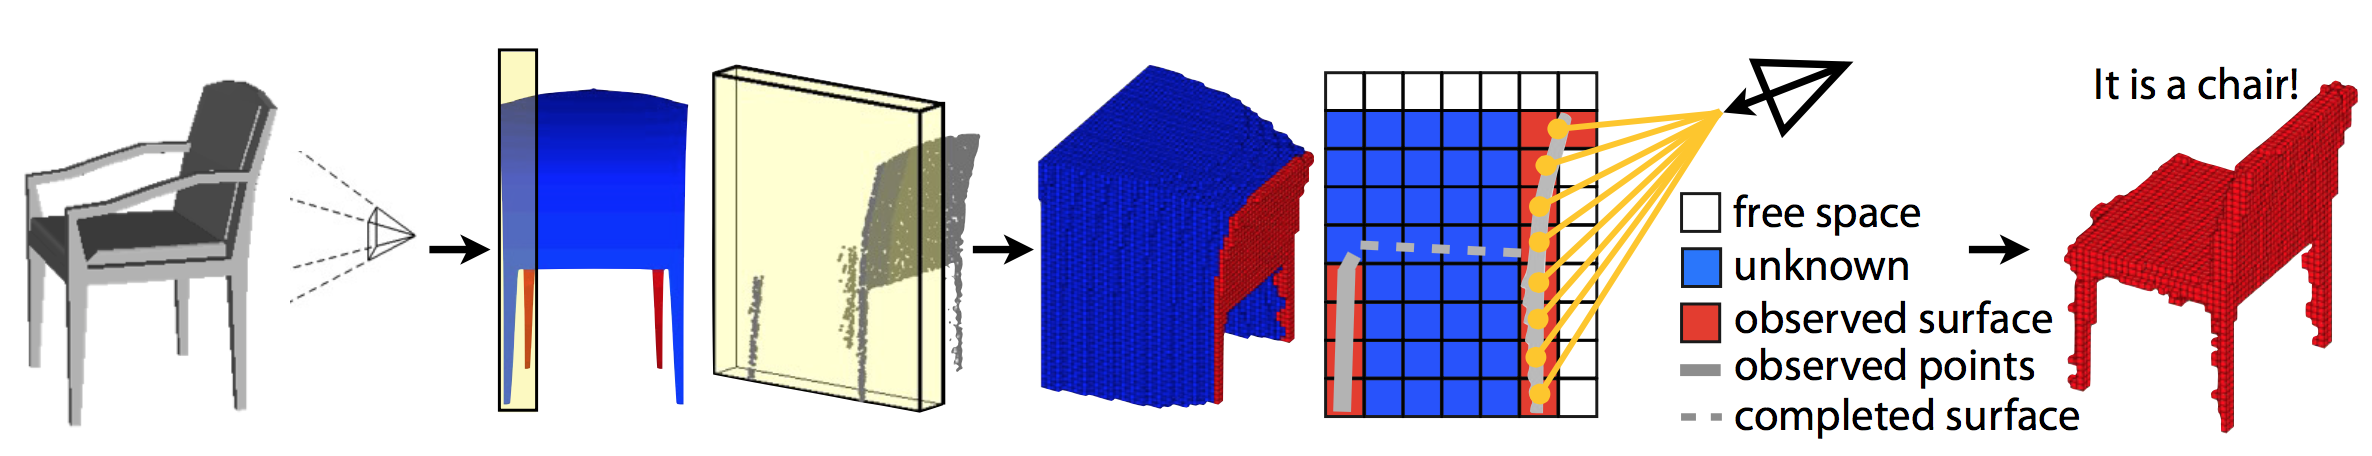
\includegraphics[width=0.5\textwidth]{algo}
	\caption{ \newline Object - Depth \& Point Cloud - Occupancy Grid - Classification. Source: \cite{shape}}
\end{figure}

Princetons ModelNet delivers every object with views from 12 different angles in .mat files; we train on all rotations to enhance recognition from 
different viwes. The data is already voxilized to 32x32x32 occupancy grids.
This data was transformed by A3 into a .hdf5 format and split into test and training set. Hdf5 compresses the set size dramatically and enables simple access.
Two methods were implemented by A1/A3 to deal with loading the data from .hdf5 files. One opens the .hdf5 and loads pieces which are passed during iterations of the generator resulting in a slower but RAM saving loader. The other, used for the final training, converts the hdf5 entirely to a numpy array providing us with a RAM expensive but much faster access to the data.

After preparing the data and its access, the VoxNet convolutional neural network model (~900.000 Parameters) is created, Figure \ref{fig:model}. For this, A1/A2 used the \textit{Python} deep learning library \textit{Keras} which runs on top of \textit{Theano}. \textit{Keras} supports 3D convolutional and max-pooling layers. 

\begin{figure}[h]
	\label{fig:model}
	\centering
	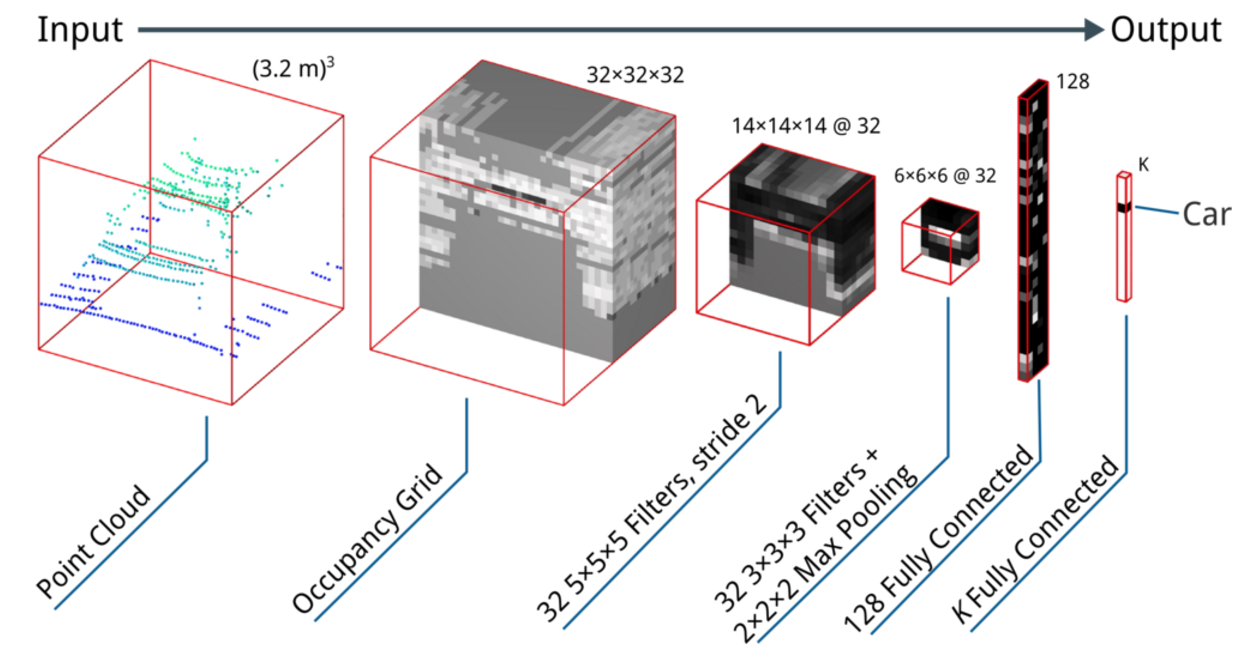
\includegraphics[width=0.42\textwidth]{model}
	\caption{VoxNet Convolution Model. Source: \cite{mature}}
\end{figure}

A training enviroment was set up by A1/A2/A3.

\section{Experiments}

The training process takes around 9 to 20 hours on a NVIDIA GTX 980TI (6GB) GPU depending on the choice of the dataset (ModelNet10/40).

\section{Results}

The papers implementation achieved verg good results for the small data set but failed to achieve the excelent score of the 
original VoxNet implementation on the larger ModelNet40. 
This is due ... TODO? WARUM? \\ 

\begin{tabular}{ |p{2.5cm}||p{2.5cm}|p{2.5cm}|  }
 \hline
 Algorithm & ModelNet10 Classification Accuracy  & ModelNet40 Classification Accuracy \\
 \hline
 VoxNet \cite{maturana_iros_2015}   & 83\% & 92\% \\
 3DShapeNets  \cite{shape}   & 77 \% & 83.5\% \\
\textbf{ETH VoxNet}    & \textbf{81.8\%}   & \textbf{82.3 \%}  \\
 \hline
\end{tabular}

\section{Conclusion}

The team successfully reimplemented a very clean and working VoxNet with comparable results.

{\small
\bibliographystyle{ieee}
\bibliography{bib}
}

\end{document}
